\scanpage{73}
and using the fact that the $\widehat M^{!}_{g_\alpha,\widehat\nu_\alpha}$ are
connected, we see that $\overset{\unsure{\deleted{\wedge}|\sim}}{M}_G^\infty=\widehat M_G\setminus M_G$
is connected as soon as \deleted{\unsure{two}} among the
factors $\widehat M^{!}_{g_\alpha,\widehat\nu_\alpha}$, there are at least
two that are of dimension $\geq1$ (using
the fact that for such an $\alpha$, we have
$M^\infty_{g_\alpha,\widehat\nu_\alpha}\ne\phi$). Thus it suffices to look at
the case where $\widehat M_G\simeq\widehat M^{!}_{g,\nu}\inserted{\simeq \unsure{\widehat M_{g,I}|M_{g,I}}}$, with
\inserted{the case where $\unsure{3g-1)+\nu=2|3(g-1)+\nu=2}$ has already been seen, so DPS $N\geq3$.}
\inserted{$(\dim M_{g,\nu}=)$} $N=\unsure{2|3}\unsure{(}g-1)+\nu\geq2$.
\deleted{In this case}, It suffices to
see that two divisors at infinity can
be joined by a chain of such divisors
of which two consecutive ones have a nonempty
intersection, given that these divisors
are themselves also connected. Now the divisors
at infinity correspond to the following \deleted{types} \inserted{MD-}graphs
\figure{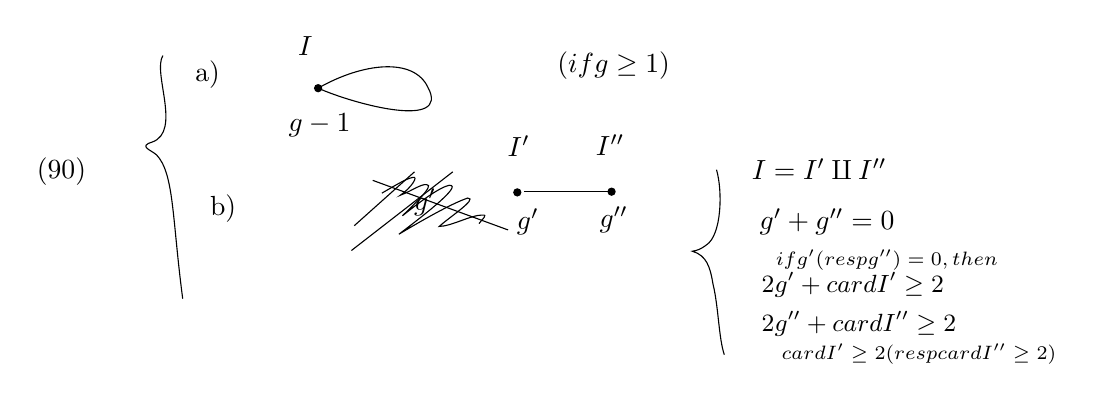
\begin{tikzpicture}[x=.009cm,y=-.009cm]
\node at (47,207) {$(90)$};
\draw (190,43)..controls(175,67)and(217,150)..(175,165)..controls(155,171)and(173,176)..(181,183)..controls(206,209)and(203,273)..(218,386);
\node at (253,70) {a)};
\fill(409,89)circle(1.5pt);
\draw(409,89)..controls(472,53)and(544,45)..(564,88)..controls(596,148)and(461,112)..(409,89);
\node at (391,30) {$I$};
\node at (411,142) {$g-1$};
\node at (826,57) {$(\text{if }g\geq1)$};
\node at (275,259) {b)};
\node at (560,250) {\deleted{$\unsure{g'}$}};
\draw (460,283)--(545,207);
\draw (499,237)..controls(515,228)and(532,217)..(542,215)..controls(552,212)and(540,230)..(525,240)..controls(541,234)and(554,224)..(562,225)..controls(575,225)and(540,257)..(528,269)..controls(548,253)and(579,229)..(594,226)..controls(615,225)and(552,273)..(523,295)..controls(548,280)and(596,252)..(620,244)..controls(636,244)and(590,274)..(580,284)..controls(596,284)and(625,268)..(640,268)..controls(650,267)and(640,274)..(636,280);
\draw (456,318)--(599,207);
\draw (486,219)--(677,289);
\fill(690,236)circle(1.5pt);
\draw(700,235)--(823,235);
\fill(823,235)circle(1.5pt);
\node at (692,171) {$I'$};
\node at (821,170) {$I''$};
\node at (705,278) {$g'$};
\node at (826,275) {$g''$};
\draw(971,204)..controls(980,235)and(978,296)..(957,310)..controls(949,316)and(944,318)..(937,319)..controls(957,325)and(962,341)..(966,365)..controls(974,398)and(974,441)..(982,465);
\node[anchor=base west] at (1007,218) {$I=I'\amalg I''$};
\node[anchor=base west] at (1018,289) {$g'+g''=0$};
\node[anchor=base west,font=\scriptsize] at (1041,339) {$\inserted{\text{if }g'\text{ (resp }g'')=0,\text{ then}}$};
\node[anchor=base west,font=\small] at (1021,377) {$\deleted{2g'+\operatorname{card}I^{\unsure{\prime}}\geq\unsure{2}}$};
\node[anchor=base west,font=\small] at (1021,432) {$\deleted{2g''+\operatorname{card}I''\geq2}$};
\node[anchor=base west,font=\scriptsize] at (1049,472) {$\inserted{\operatorname{card}I'\geq2\text{ (resp }\operatorname{card}I''\geq2\text{)}}$};
\end{tikzpicture}}
\margin{72}
